\section{Evaluation}

\subsection{Experimental Environment}
本論文では次のマシンを用いて評価する。

CPUはIntel Core i7 2600 3.40GHz、
4GB*2のメモリ、GPUはGeForce GTX680を用いる。
KernelはLinux kernel 3.16.0を用い、ディストリビューションはUbuntu 14.04である。
CUDAランタイムはcuda-6.0 or Gdev、GPUドライバはNVIDIAの331.62を用いる。

より高精度な測定を行うために、ユーザ空間ではclock\_gettimeを用いて直接TSCレジスタにアクセスして測定する。
カーネル空間ではsched\_clock()を用いて計測する。

\subsection{Interrupt intercept overhead}
Interrupt interceptのオーバヘッドの測定を行う。
本評価では、GPUドライバはnouveauを用いる。
割り込み処理は、各割り込みの種類によって、処理時間が異なり、その分布は一様ではないため、単に測定して平均をとっても比較ができない。
そのため各割り込みの種類の判別のためにNouveauを用いて、割り込みの種類が同一のもので、カーネル内のdo\_IRQ関数内でハンドラが呼ばれてから終了までの時間を測定し
どの程度のオーバヘッドで割り込みの盗聴及び、盗聴した割り込みの識別ができるかどうかを測定する。

\begin{figure}[t]
\begin{center}
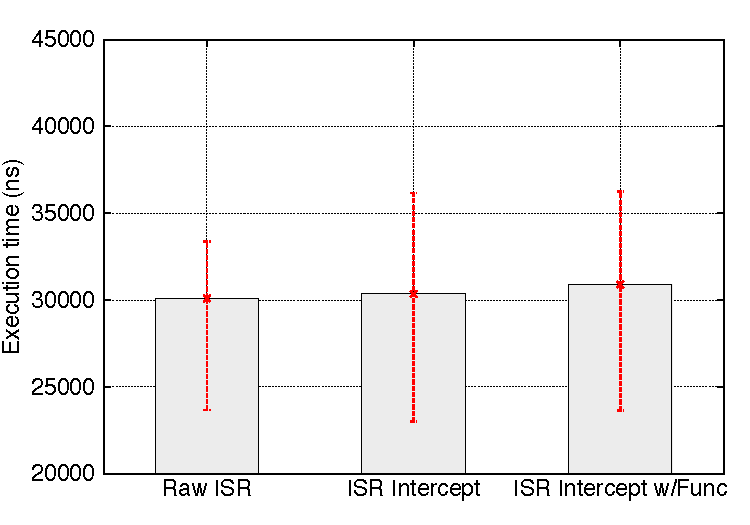
\includegraphics[width=0.4\textwidth]{graph/interrupt.pdf}
\caption{Interrupt intercept overhead}
\end{center}
\label{fig:irq_overhead}
\end{figure}

Figure \ref{irq_overhead}は上記設定で測定した結果である。
Raw ISRは通常のルーチンで実行されるISR、ISR Interceptは割り込みを盗聴するのみ、ISR intercept w/Funcは盗聴した上でその割り込みがどの割込みか識別しスケジューラを立ち上げる機能を実行した場合である。
それぞれ1000回の測定で平均値を取り、最小値と最大値についてエラーバーで示している。
この図から見て取れるように、オーバヘッドは確実に存在する。
ISR Interceptだと247nsのオーバヘッドであり、
ISR Intercept w/Funcでも790nsのオーバヘッドである。
この数値は直感的に考えると小さくシステム自体に影響を及ぼすほどではないと考えられる。
しかしその積み重ねによっては影響を与えることは考えなければならない。

\subsection{Interrupt raised overhead}
本稿では割込み立ち上げのためのオーバヘッドを測定する。
割込み立ち上げは2つのAPIの呼び出しを必要とする。
一つはcuCtxCreateを呼び出したあとに呼び出すrtx\_nvrm\_init()である。
もう一つは同期したいタイミング(e.g. カーネルラウンチ後)に呼び出すrtx\_nvrm\_notify()である。
スケジューリングを行わないVanillaな状態ではこれらのAPIは必要ではないものであるため、これらのAPIにかかった時間はすべてオーバヘッドとなる。

そのためこれらのオーバヘッドの計測を行う。
計測はAPIの呼び出しから戻るまでを測定する。

\begin{figure}[!t]
\begin{center}
\subfigure[Part of Initialize]{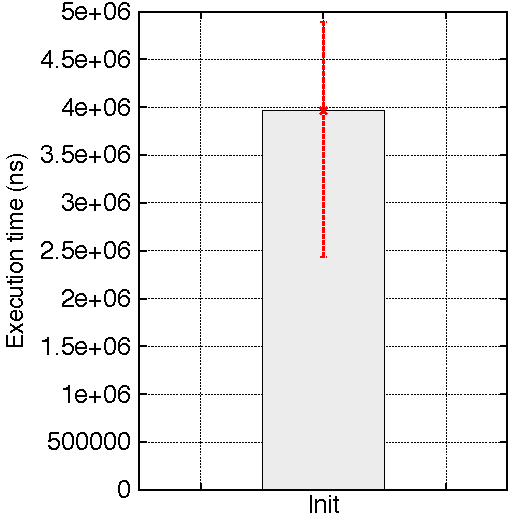
\includegraphics[width=0.23\textwidth]{graph/irq_rise_init.pdf}}\subfigure[Part of notify]{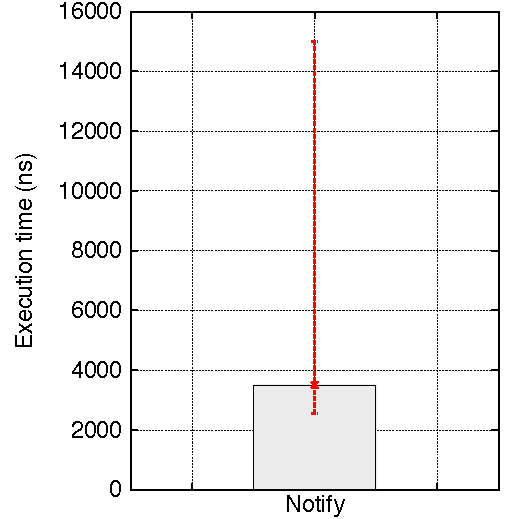
\includegraphics[width=0.23\textwidth]{graph/irq_rise_notify.pdf}}
\caption{Interrupt raised method overhead}
\label{fig:irq_rise_overhead}
\end{center}
\end{figure}

結果をFigure \ref{fig:irq_rise_overhead}に示す。
InitializeはIndirect Bufferはプロセスが立ち上がるたびに、
コマンド送信用のIndirect Bufferの確保や各エンジンの登録のために呼び出される必要がある。
Notifyはカーネル実行後や非同期メモリコピー実行後のような実際に割込みを発生させたいタイミングで呼び出される。
これらはioctlシステムコールによってユーザ空間とカーネル空間をまたいでる影響か、実行時間のバラ付きが大きく出ている。

Initializeは比較的時間がかかっているが、1プロセスにつき一度しか呼ばれないため、アプリケーション全体への影響は少ないと考えられる。
Notifyに関してはそれほど時間がかかっておらず、同期待ちの間に実行されるべき処理なため、こちらもアプリケーション全体への影響は少ないと考えられる。

\subsection{Overhead}


\subsection{Compare the prior work}
